\documentclass[12pt]{scrartcl}

\usepackage{fontspec}
\usepackage{polyglossia}
\setdefaultlanguage{russian}
\newcommand{\docfont}{Times New Roman}
\setmainfont[Ligatures=TeX]{\docfont}
\newfontfamily\cyrillicfont[Ligatures=TeX]{\docfont}
\newfontfamily\cyrillicfontsf[Ligatures=TeX]{\docfont}
\newfontfamily\cyrillicfonttt[Ligatures=TeX]{\docfont}

\usepackage{amsmath,amsfonts,amsthm,amssymb} % nice math symbols
\newtheorem{definition}{Определение}
\usepackage{hyperref}

\hypersetup{%
	pdfencoding=auto,
	pdfauthor={Александр Панов},
	pdftitle={Операции в знаковой картине мира}
}
\usepackage{csquotes}
\usepackage{graphicx}
\graphicspath{{../../images/}}

\usepackage[plain]{algorithm}
\usepackage[noend]{algpseudocode}

\usepackage[
%	autolang=hyphen,
	language=auto,
	autolang=other,
	backend=biber,
	style=gost-numeric
]{biblatex}
\addbibresource{../../biblio/library.bib}
\DeclareSourcemap{
	\maps[datatype=bibtex, overwrite]{
		\map{
			\step[fieldset=langid, fieldvalue=english]
			\step[fieldset=doi, null]
			\step[fieldset=issn, null]
			\step[fieldset=isbn, null]
			\step[fieldset=url, null]
			\step[fieldsource=language, fieldset=langid, origfieldval]
		}
	}
}

\linespread{2}

\title{Семиотический способ представления знаний: операции в знаковой картине мира}
\author{Осипов~Г.\,С., Панов~А.\,И.\\
	{\large\slshape ФИЦ ИУ РАН, пр. 60-летия Октября, 9, gos@isa.ru}}

\begin{document}
%	\affil{ФИЦ ИУ РАН}
	
	\maketitle{}
	\begin{abstract}
		В работе представлен новый способ представления знаний как на уровне сенсорных данных так и на уровне концептуальной информации, - знаковая картина мира. Базовым элементом картины мира является четырехкомпонентная структура - знак, строение которого подтверждается как психологическими теориями, так и нейрофизиологическими данными. В работе представлены принципы работы математической структуры - каузальной матрицы, которая описывает строение компонент знака. Предложены алгоритмы пополнения отношений на множестве знаков, определены операции в знаковой картине мира, который моделируют важные психологические особенности поведения человека.
		\par\bigskip
		\textit{Ключевые слова}: знаковая картина мира, образ, значение, личностный смысл, каузальная матрица, семиотическая сеть.
	\end{abstract}
	
	
	
	\section*{Введение}
	Про постановку задачи \cite{Osipov2014c,Osipov2015d}.
	
	Психологические и нейрофизиологические основания трехкомпонентной структуры знака (Станович, Гроссберг и др. более новые).
	
	\section{Картина мира}

	Про компоненты знака, функции связывания и три типа картин мира.
	
	Введем два знака,~которые мы будем рассматривать на протяжении всей статьи в качестве примеров, иллюстрирующих положения, которые приводятся в настоящей работе (квадрат, выстрел).
	
	
	\section{Строение компонент знака}
	
	Далее рассмотрим структуру компонент знака на примере образной компоненты, которая участвует в актуализации знака, выделении представления об опосредуемом объекте или процессе на основе поступающей из внешней среды сенсорной информации и регистрируемой внутренними сенсорами моторной информации. До именования знак будем называть протознаком или признаком.
	
	Предположим, что во входном потоке данных выделена последовательность $(x_1,x_2,\dots,x_h)$ длины $h$ векторов действительных чисел от 0 до 1, которые будем называться \textit{событиями}. Каждое событие $x_t$ длины $q$ представляет собой запись выходов от $q$ сенсоров, а каждый элемент события означает уверенность в срабатывании данного сенсора. Например, событие $(0.1, 0.9, 0.9)$ поступает с трех сенсоров - датчиков красного, синего и зеленого света - и означает, что уверенность в срабатывании датчика красного света составляет 10\%, а синего и зеленого - по 90\%.
	
	Образная компонента знака должна по входной последовательности данных определить, присутствует ли (закодирован ли) опосредуемый объект или процесс в этой последовательности. Для этого мы будем кодировать характерные признаки объекта или процесса в специальной структуре - каузальной матрице $z=(e_1,e_2,\dots,e_h)$ размерности $q$ на $h$, где $q$ - размерность входных событий, а $h$ - длина последовательности входных событий. При этом каждый столбец $e_t$ каузальной матрицы является битовым вектором длины $q$ и кодирует те признаки (которым соответствуют 1), которые необходимо должны присутствовать во входном событии в момент времени $t$, чтобы опосредуемый объект или процесс мог быть распознан во входном потоке данных, т.е. задают множество одновременных характерных признаков. Например, образу знака $s$, опосредующему объект <<квадрат>>, может соответствовать каузальная матрица 	\[z=((1,0,1,1,0),(1,1,0,1,0),(1,1,0,0,1),(1,0,1,0,1)),\]
	где первая строчка является характеристическим вектором информации с датчика углов на изображении, вторая - с датчика положения визуального сенсора (верхнее положение), третья - нижнее положение сенсора, четвертая - левое положение сенсора, пятая - правое положение (см. рис.\ref{fig:square}).

	\begin{figure}
		\label{fig:square}
		\centering
		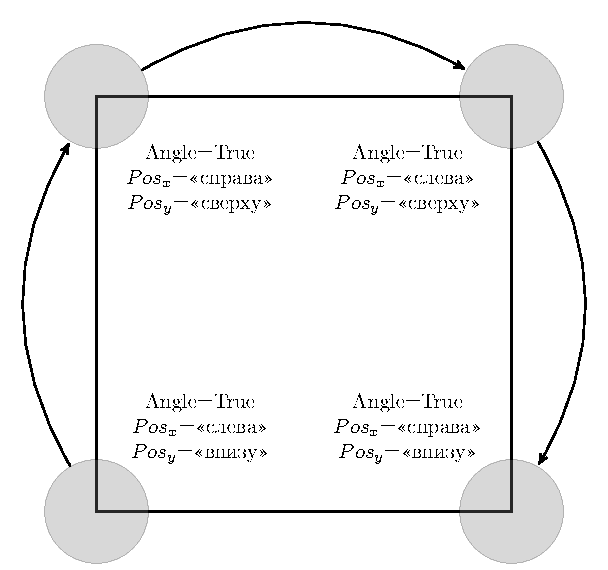
\includegraphics[width=0.5\textwidth]{examples/square}
		\caption{Визуальная интерпретация каузальной матрицы}		
	\end{figure}

	Образу каждого знака может соответствовать несколько каузальных матриц, которые задают различные проявления опосредуемого объекта или процесса. Весь кортеж каузальных матриц образа знака $s$ будем обозначать как $Z^p(s)$. 
	
	Случай, когда характерными признаками образа данного знака выступают данные с сенсоров, является частным. В более общей постановке, признаками для образа знака служат другие знаки, которые опосредуют эти характерные признаки. Таким образом, мы можем сопоставить образу знака $s$ множество $S_p(s)$ мощности $q$, каждому элементу которого соответствует номер строчки каузальной матрицы $z$ размера $q$ на $h$, т.е. каждому признаку $s_i\in S_p(s)$ соответствует характеристический битовый вектор, задающий на местах 1 те моменты времени, когда данный признак должен присутствовать во входных данных, чтобы успешно актуализировать знак (распознать образ знака) $s$. 
	
	Для уточнения определения множества $S_p(s)$ введем семейство бинарных отношений $\{\sqsubset_p,\sqsubset_p^1,\sqsubset_p^2,\dots\}$, определённых на декартовом произведении $S\times S$. Будем считать, что знак $s_i$ \textit{поглощается} знаком $s$ по образу, $(s_i,s)\in\sqsubset_p$ или $s_i\sqsubset_p s$, в том случае, если $s_i\in S_p(s)$. Если известно, что знаку $s_i$ соответствует 1 в $t$-м столбце некоторой каузальной матрицы $z\in Z^p(s)$ знака $s$, то мы будем использовать уточненное отношение $\sqsubset_p^t\subset \sqsubset_p$.
	
	\subsection{Актуализация образной компоненты знака}
	
	Кратко опишем работу алгоритма актуализации знака (распознавания образа знака) по рис.~\ref{fig:percept}. Будем считать, что образы знаков сгруппированы по схожести множеств $S_p(s)$ в узлы, которые организованы в иерархические структуры (подробнее см. \cite{Panov2014d}).
	
	\begin{figure}
		\centering
		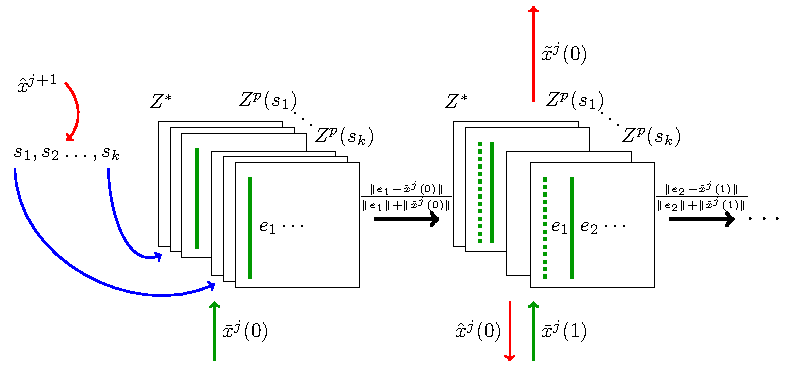
\includegraphics[width=0.8\textwidth]{algo/perception}
		\caption{Схема алгоритма актуализации знака}
		\label{fig:percept}		
	\end{figure}

	Вычислительный цикл распознавания в узле уровня $j$ начинается с определения начального состояния узла при помощи предсказывающего воздействия с верхнего уровня иерархии - вектора ожиданий $\hat x_i^{j+1}(\tau_s)$ (шаги \ref{alst:init_start}--\ref{alst:init_end}) в момент времени $\tau_s$. Начальное состояние определяется как подмножество таких знаков, образы которых предсказываются на основе состояния узла верхнего уровня. Первая константа $c_1$ определяет порог предсказываемого веса распознаваемых образов, выше которого соответствующие каузальные матрицы попадают во множество активных матриц $Z^*$ (шаг \ref{alst:select_f}). Далее производится отбор тех каузальных матриц из множества активных, для которых обычное расстояние по норме $\|x\|=\sum_i |x_i|$ первого столбца $\bar z_1^r$ от входного вектора $\bar x_i^j$ в начальный момент времени не превышает второй константы $c_2$ (шаг \ref{alst:select_z}). Обновленное множество полученных таким образом активных каузальных матриц является текущим состоянием узла (шаг \ref{alst:init_state}). На основе активных каузальных матриц методом голосования вычисляется выходной вектор узла  в начальный момент времени $\bar x_i^{j*}(\tau_s)$ (шаги \ref{alst:init_calc_out2} -- \ref{alst:init_calc_out3}).

	\linespread{1}
	\begin{algorithm}[H]
		\label{alg:automato}
		\begin{algorithmic}[1]
					\Require $\tau_s, \hat x^{j+1}(\tau_s)$, $\omega^j$ - функция входов.
		\Ensure $\varphi^j$ - функция ожиданий, $\vec\eta^j$ - функция выходов.

		\State $F^*=\varnothing,Z^*=\varnothing,t=0$; 
		\State $c_1\in(0,1), c_2\in(0,1)$;

		\Statex \Comment{определение начального состояния}
				
		\ForAll{компонент $\hat x_k^{j+1}$ вектора $\hat x^{j+1}(\tau_s)=(\hat x_1^{j+1},\hat x_2^{j+1},\dots,\hat x_l^{j+1})$} \label{alst:init_start}
			\If{$\hat x_k^{j+1}{\ge}c_1$} \label{alst:select_f}
				\State $F^*=F^*\cup\{s_k\}$;
			\EndIf
		\EndFor
		
		\State $\bar x(0):=\omega^j(\tau_s)$;
		
		\ForAll{знаков $s_k\in F^*$}
			\ForAll{каузальных матриц $z\in Z^p(s_k)$}
				\If{$\frac{\|e_1-\bar x^j(0)\|}{\|e_1\|+\|x^j(0)\|}<c_2$} \label{alst:select_z}
					\State $Z^*:=Z^*\cup\{z\}$;
				\EndIf
			\EndFor
		\EndFor
		
		\State $Z^*$ - начальное состояние узла; \label{alst:init_state}
		\State $\bar N=(|\{z|z\in Z^*,z\in Z^p(s_1)\}|,\dots,|\{z|z\in Z^*,z\in Z^p(s_l)\}|)$; \label{alst:init_calc_out2}
		\State $\eta(0):=\tilde x^j=W(\bar N)$; \label{alst:init_calc_out3}
		\State $\varphi^j(0):=\hat x^j=W(\sum_{s_k\in F^*}\hat x_k^{j+1}\sum_{z\in Z^*}e_2(z))$;\label{alst:init_control}
		\label{alst:init_end}
			\algstore{algst:store1}
		\end{algorithmic}
	\end{algorithm}
	\linespread{2}

	Вектор ожиданий $\hat x_i^j(\tau_s+1)$ определяется как нормированный вектор, $s$-ый компонент которого равен сумме всех $s$-ых элементов вторых колонок активных каузальных матриц с весами, соответствующими элементам вектора ожиданий $\hat x_i^{j+1}(\tau_s)$ (шаг \ref{alst:init_control}). Т.к. используется представление о будущем входном сигнале (вторая колонка матриц предсказания), то $\hat x_i^j(\tau_s+1)$ играет роль предсказывающего вектора для нижнего уровня иерархии.

	\linespread{1}
	\begin{algorithm}[H]
		\begin{algorithmic}[1]
			\algrestore{algst:store1}
				\Statex \Comment{основной цикл}
	
	\State $t=1$;
	\While{$t\leqslant{h_i^j}-1$} \label{alst:cycle_start}
		\State $\bar{x}_i^j:=\omega(\tau_s+t)$;
	
		\ForAll{матриц предсказания $Z_r^k$ из множества $Z^*$}
			\If{$\frac{\|\bar{z}_{t+1}^r-\bar{x}_i^j\|}{\|\bar{z}_{t+1}^r\|+\|\bar{x}_i^j\|}\geqslant{c_2}$} \label{alst:update_z}
				\State $Z^*:=Z^*\setminus\{Z_r^k\}$;
			\EndIf
		\EndFor
	
		\State $\varphi_i^j(\bar x_i^j,\hat{x}_i^{j+1}(\tau_s)) := Z^*$; 
		\State $\bar N=(|\{Z_r^1|Z_r^1\in Z^*\}|,\dots,|\{Z_r^{l_i^j}|Z_r^{l_i^j}\in Z^*\}|)$; \label{alst:calc_out1}
		\State $\eta(Z^*)=\bar{x}_i^{*j}:=W(\bar N)$; \label{alst:calc_out3}
	
		\State $t=t+1$;
		\If{$t\leqslant{h}_i^j-2$}
			\State $\hat{x}_i^j:=W(\sum_{\hat f_k\in\hat F^*}\hat x_{ik}^{j+1}\sum_{Z_r^k\in Z^*}\bar z_t^r)$; \label{alst:calc_state1}
		\EndIf
	\EndWhile \label{alst:cycle_end}
	
	\Return $\varphi_{i\Delta t}^j,\vec\eta_{i\Delta t}^j$.
		\end{algorithmic}
	\end{algorithm}
	\linespread{2}
		
	После определения начального состояния начинает выполняться тело основного цикла, в котором до тех пор, пока время не превысит характерное время узла $h_i^j$ (размер каузальных матриц, входящих в него образов знаков) повторяется вычисление выходного вектора и состояния в следующий момент времени (шаги \ref{alst:cycle_start}--\ref{alst:cycle_end}). В начале обновляется состояние, т.е. множество активных каузальных матриц $Z^*$, за счёт удаления тех матриц, соответствующие столбцы которых достаточно сильно отличаются от текущего входного вектора $\bar x_i^j$ (шаг \ref{alst:update_z}). Далее методом голосования по количеству матриц в множестве активных каузальных матриц, отвечающих за соответствующий образ, вычисляется выходной вектор $\bar x_i^{j*}$ (шаги \ref{alst:calc_out1}--\ref{alst:calc_out3}).

	
	В завершение тела основного цикла вычисляется выходной вектор ожиданий в следующий момент времени $\hat x_i^j(\tau_s+t+1)$. Вектор ожиданий равен нормированному вектору, элементы которого равны сумме элементов столбцов всех активных кауазальных матриц, соответствующих текущему моменту времени с учётом весов начального вектора ожиданий $\hat x_i^{j+1}(\tau_s)$ (шаг \ref{alst:calc_state1}).

	\subsection{Каузальная сеть}
	
	Введем специальную процедуру $\Lambda_p: 2^Z\rightarrow 2^{\mathbb N}\times 2^{\mathbb N}$, которая каждому кортежу каузальных матриц $Z^p(s)\subset Z$ образа знака $s$ ставит в соответствие два не пересекающихся подмножества индексов собственных столбцов $I^c\subset\mathbb N, \forall i\in I^c\ i\leq h$ (индексы столбцов условий) и $I^e\subset\mathbb N, \forall i\in I^e\ i\leq h$ (индексы столбцов эффектов): $\Lambda_p(Z^p(s))=(I^c,I^e), I^c\cap I^e=\varnothing$. Например, если для множества матриц $Z=\{((1, 0), (0, 1))\}$ процедура $\Lambda_p$ выдает два множества $\{1\}$ и $\{2\}$, то это означает, что появление признака, соответствующего первой строчке матрицы, вызывает появление признака, соответствующего второй строчке. Процедура $\Lambda_p$ по сути является функцией установления причинно-следственного отношения на множестве входных событий и может реализовываться различными способами, в т.ч. на основе алгоритмов Норриса, FCO и др. (см. \cite{Kuznetsov2001})
	

	В том случае, когда для матриц $Z^p(s)$ образа знака $s$ множество столбцов эффектов пусто $I^e=\varnothing$, т.е. когда по данному множеству каузальных матриц не возможно однозначно определить, какие события всегда предшествуют другим, мы будем считать, что причинно-следственная связь не установлена и знак опосредует некоторый объект или ситуацию. В противном случае будем считать, что знак опосредует некоторое действие или процесс, результат которого кодируется в столбцах эффектов, а условие - в столбцах условий. 

	\begin{figure}[H]
		\centering
		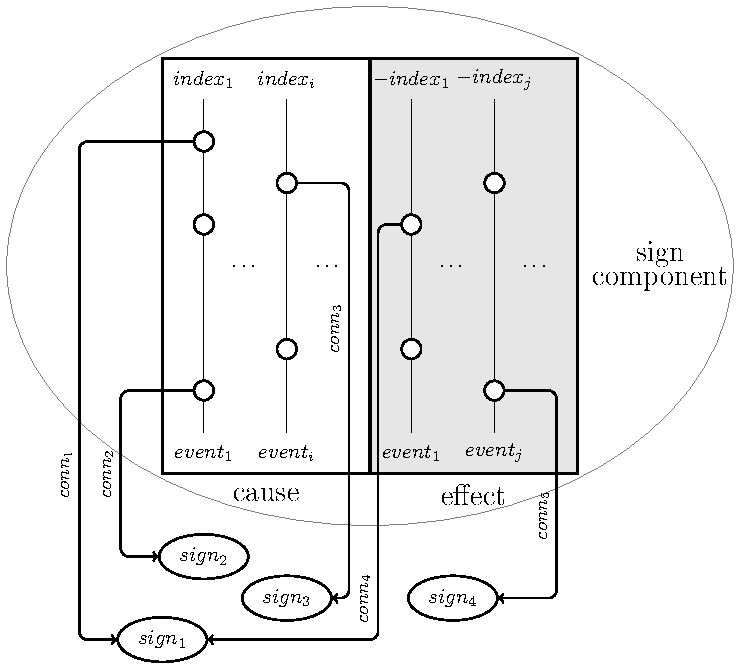
\includegraphics[width=0.6\textwidth]{automata/caus_matr}
		\caption{Схема каузальной матрицы}	
		\label{fig:caus_matr}	
	\end{figure}
	
	Справедливы следующие утверждения относительно свойств процедуры $\Lambda_p$:
	\begin{itemize}
		\item $I^c\cap I^e=\varnothing$ --- столбец матрицы предсказания не может быть одновременно и условием и эффектом,
		\item $|I^c\cup I^e|=h$ --- столбец матрицы предсказания является либо условием либо эффектом,
		\item $I^c\not = \varnothing$ --- среди столбцов матрицы предсказания должен быть хотя бы один столбец условий, в то время как эффектов может и не быть (в случае объектных признаков),
		\item $\forall i\in I^e, j\in I^c\ i>j$ --- все условия предшествуют эффектам по времени.
	\end{itemize}
	
	Схема каузальной матрицы, с учетом выше сказанного, приведена на рис. \ref{fig:caus_matr}.
	
	Теперь введем понятие каузальной сети, которая будет определять гетерархию на множестве образов. Каузальная сеть $W_p=\langle V_p, E_p \rangle$ - является помеченным ориентированным графом, в котором
	\begin{itemize}
		\item каждому узлу $v\in V_p$ ставится в соответствие кортеж казуальных матриц $Z^p(s)$ образа некоторого знака $s$, что будем обозначать как $v\rightarrow Z^p(s)$;
		\item ребро $e=(v_1, v_2)$ принадлежит множеству ребер графа $E$, если $v_1\rightarrow Z^p(s_1), v_2\rightarrow Z^p(s_2)$ и $s_1\in S_p(s_2)$, т.е. если знак $s_1$ поглощается знаком $s_2$;
		\item каждому ребру графа $e=(v_1, v_2), v_1\rightarrow Z^p(s_1), v_2\rightarrow Z^p(s_2)$ ставится в соответствие метка $\epsilon=(\epsilon_1,\epsilon_2,\epsilon_3)$ - кортеж трех натуральных чисел:
		\begin{itemize}
			\item $\epsilon_1$ - индекс исходной матрицы в кортеже $Z^p(s_1)$, может принимать специальное значение 0, если исходными могут служить любые матрицы из кортежа;
			\item $\epsilon_2$ - индекс целевой матрицы в кортеже $Z^p(s_2)$, строка которой ставится в соответствие признаку $s_1$;
			\item $\epsilon_2$ - индекс столбца в целевой матрице, в которой в соответствующей признаку $s_1$ строке стоит 1, может принимать положительные значения (столбцы условий) и отрицательные (столбцы эффектов).
		\end{itemize}		
	\end{itemize}
	
	Пример такой сети изображен на рис. \ref{fig:caus_net}.
	
	Аналогичным образом определяются каузальные сети для остальных компонент знака - для значения и личностного смысла. Для каждого знака $s$ задаются множества $S_m(s)$ и $S_a(s)$, т.е. определяются семейства отношений $\{\sqsubset_m,\sqsubset_m^1,\sqsubset_m^2,\dots\}$ и $\{\sqsubset_a,\sqsubset_a^1,\sqsubset_a^2,\dots\}$. Множество $S_m(s)$ интерпретируется как ролевой состав знака $s$, например, элементы подкласса или роль действия. Множество $S_a(s)$ интерпретируется как мгновенный компонентный состав некоторой ситуации, наблюдаемой и переживаемой субъектом, носителем картины мира, в настоящее время. Аналогично определяются множества $Z^m(s)$, $Z^a(s)$, процедуры $\Lambda_m$ и $\Lambda_a$.
	
	\begin{figure}[H]
		\centering
		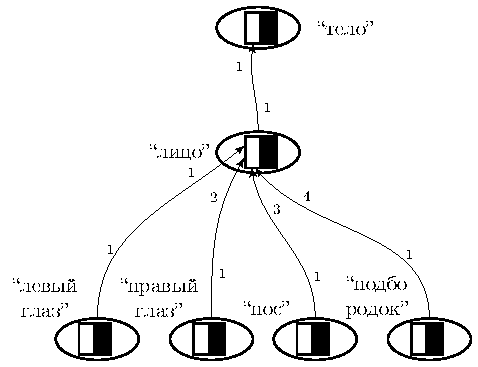
\includegraphics[width=0.5\textwidth]{automata/caus_net}
		\caption{Схема каузальной сети. Здесь каузальные матрицы изображены в виде квадратов, столбцы условий - левая белая часть квадрата, столбцы эффектов - черная правая часть квадратов. Метка $\epsilon_1$ отображается в начале каждой стрелки, метка $\epsilon_2$ определяется как номер квадрата, к которому идет стрелка, а метка $\epsilon_3$ отображается в конце каждой стрелки.}
		\label{fig:caus_net}		
	\end{figure}
	
	\section{Семиотическая сеть}
	
	Далее определим три семейства бинарных отношений на множестве знаков, которые  генерируются на основе структуры фрагментов трех типов каузальных сетей, к которым принадлежат соответствующие компоненты знаков.
		
	\subsection{Отношения на множестве образов}	
	
	Начнем с определения отношений на множестве знаков, генерируемых на основе каузальной сети на образах. Для этого потребуется определения равенства, сходства, включения и противопоставления двух каузальных матриц:
	
	\begin{definition}
		Две каузальных матрицы $z_1$ и $z_2$ равны ($z_1=z_2$) тогда и только тогда, когда размерности матриц равны, множества индексов столбцов эффектов и условий совпадают $\Lambda({z_1})=\Lambda({z_2})$ и каждый битовый вектор $e_t^1$, столбец матрицы $z_1$, равен соответствующему по порядку битовому вектору $e_t^2$, столбцу матрицы $z_2$.
	\end{definition}
	
	\begin{definition}
		Две каузальных матрицы $z_1$ и $z_2$ схожи ($z_1\sim z_2$) тогда и только тогда, когда  существуют такие два битовых вектора $e_i$ и $e_j$, столбца матриц $z_1$ и $z_2$, что они равны $e_i=e_j$ и они одновременно являются либо столбцами условий $i\in I_c(z_1), j\in I_c(z_2)$, либо столбцами эффектов $i\in I_e(z_1), j\in I_e(z_2)$.
	\end{definition}
	
	\begin{definition}
		Каузальная матрица $z_1$ включена в каузальную матрицу $z_2$ ($z_1\subseteq z_2$) тогда и только тогда, когда  для любого битового вектора $e_i$, столбца матрицы $z_1$, существует битовый вектор $e_j$, столбец матрицы $z_2$, такой, что $e_i | e_j=e_j$ ($|$ - операция побитового <<или>>) и они одновременно являются либо столбцами условий $i\in I_c(z_1), j\in I_c(z_2)$, либо столбцами эффектов $i\in I_e(z_1), j\in I_e(z_2)$.
	\end{definition}
	
	\begin{definition}
		Две каузальных матрицы $z_1$ и $z_2$ противопоставлены друг другу ($z_1\perp z_2$) тогда и только тогда, когда размерности матриц равны, множества индексов столбцов эффектов и условий совпадают $\Lambda({z_1})=\Lambda({z_2})$ и каждый битовый вектор $e_t^1$, столбец матрицы $z_1$, не имеет пересечения с соответствующим ему по порядку битовым вектором $e_t^2$, столбцом матрицы $z_2$, т.е. $e_t^1\& e_t^2=e_0$, где $\&$ - операция побитового <<и>>, а $e_0$ - нулевой вектор той же длины, что и вектора $e_t^1$ и $e_t^2$.
	\end{definition}
	
	На основе этих определений введем четыре отношения на множестве знаков $S$.
	\begin{definition}
		Пара знаков  $s_1$ и $s_2$ принадлежит \textbf{отношению эквивалентности по образам} $R_1^p$, $(s_1,s_2)\in R_1^p$, если мощность кортежа $S_p(s_1)=(z_1^1,z_2^1,...)$ равна мощности кортежа $S_p(s_2)=(z_1^2,z_2^2,...)$ и каждая каузальная матрица первого кортежа равна соответствующей по порядку матрице второго кортежа, т.е. $|S_p(s_1)| = |S_p(s_2)|, \forall z_t^1\in S_p(s_1)\ \exists z_t^2\in S_p(s_2): z_t^1=z_t^2$.
	\end{definition}
	
	\begin{definition}
		Пара знаков  $s_1$ и $s_2$ принадлежит \textbf{отношению сходства по образу} $R_2^p$, $(s_1,s_2)\in R_2^p$, если для каждой каузальной матрицы $z_i$ кортежа $S_p(s_1)$ в кортеже $S_p(s_2)$ найдется такая матрица $z_j$, что $z_i$ будет схожа с $z_j$, т.е. $\forall z_i\in S_p(s_1)\ \exists z_j\in S_p(s_2): z_i\sim z_2$.
	\end{definition}
	
	\begin{definition}
		Пара знаков  $s_1$ и $s_2$ принадлежит \textbf{отношению включения по образу} $R_3^p$, $(s_1,s_2)\in R_3^p$, если для каждой каузальной матрицы $z_i$ кортежа $S_p(s_1)$ в кортеже $S_p(s_2)$ найдется такая матрица $z_j$, что $z_i$ будет включена в $z_j$, т.е. $\forall z_i\in S_p(s_1)\ \exists z_j\in S_p(s_2): z_i\subseteq z_2$.
	\end{definition}

	\begin{definition}
		Пара знаков  $s_1$ и $s_2$ принадлежит \textbf{отношению противопоставления по образу} $R_4^p$, $(s_1,s_2)\in R_4^p$, если мощность кортежа $S_p(s_1)=(z_1^1,z_2^1,...)$ равна мощности кортежа $S_p(s_2)=(z_1^2,z_2^2,...)$ и каждая каузальная матрица первого кортежа противопоставлена соответствующей по порядку матрице второго кортежа, т.е. $|S_p(s_1)| = |S_p(s_2)|, \forall z_t^1\in S_p(s_1)\ \exists z_t^2\in S_p(s_2): z_t^1\perp z_t^2$.
	\end{definition}
	
	
	
		
	\subsection{Отношения на множестве значений}	
	Ролевые отношения
	\subsection{Отношения на множестве личностных смыслов}	
	Ситуационное отношения и сценарное отношение.
	
	\subsection{Семиотическая сеть}
	Будем называть \textit{семиотической сетью} пятерку $\Omega=\langle W_p, W_m, W_a, R_n, \Theta \rangle$, где
	\begin{itemize}
		\item $W_p, W_m, W_a$ - соответственно каузальные сети на множестве образов, значений и личностных смыслах,
		\item $R_n$ - семейство отношений на множестве знаков, сгенерированных на основе трех каузальных сетей, т.е. $R_n=\{R_p, R_m, R_a\}$,
		\item $\Theta$ - семейство операция на множестве знаков, которые будут определены ниже.
	\end{itemize} 
	

	\section{Операции в семиотической сети}
	Операции осуществляется в одной сети --- как это сказывается на компонентах знака в другой сети, как они преобразуются. Содержательной описание операций. Пример: обобщение на сети образов для знаков <<яблоко>> и <<апельсин>> общее значение не включает в себя действие <<чистить>>, т.к. не присутствуют все необходимые признаки в обобщенном образе (нет ссылки на знак <<кожура>>).
	
	\subsection{Операция обобщения}
	
	\subsection{Операция замыкания по значению}
	
	\subsection{Операция агглютинации смыслов}
	
	\section*{Заключение}
	
	\printbibliography
\end{document}